 

\documentclass{article}

\usepackage{fullpage}
\usepackage{graphicx}


\title{Sesión 4: Superposición de señales DC y AC}
\date{}
\author{Pablo Cuesta Sierra. Grupo 1201. Puesto 10.}



\begin{document}

\maketitle
\begin{center}
\section*{MONTAJE EXPERIMENTAL}
\end{center}
\textbf{Construya el circuito en el panel de la entrenadora. La señal de tensión continua $V_1$ de $10V$ DC será la proporcionada por la fuente S1. La señal de tensión sinusoidal $V_2$ se obtendrá del generador de funciones, fijando inicialmente una amplitud de 2V y una frecuencia de 1kHz. Conectaremos con un cable la señal a la entrenadora.}
\bigskip

\begin{center}
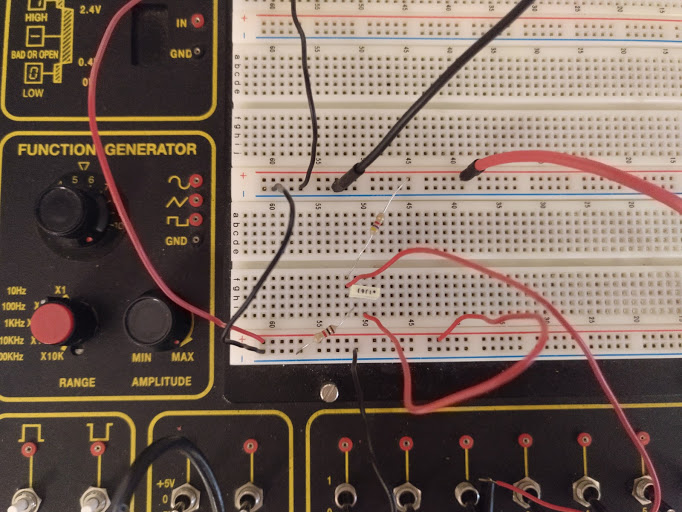
\includegraphics[scale=0.4]{circuito}\\
Circuito montado en la entrenadora.
\end{center}

\textbf{Utilice el canal 1 del osciloscopio en modo de acoplamiento DC y mida la diferencia de tensión en  el  nodo A ($V_A$). Represente su  valor  en  función  del  tiempo, indicando  los  valores máximos y mínimos que alcanza la señal.\\
Mida el valor promedio de la señal utilizando el menú de medida del osciloscopio.}

La diferencia de tensión en el nodo A, correspondiente a la fuente continua, se obtiene con el valor promedio de $V_A$. Incluyo a continuación las medidas de los valores medio, máximo y mínimo. 

\begin{center}
\includegraphics[scale=0.203]{vmedio1}
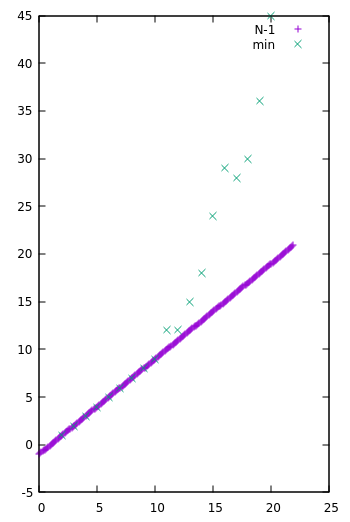
\includegraphics[scale=0.2]{min}
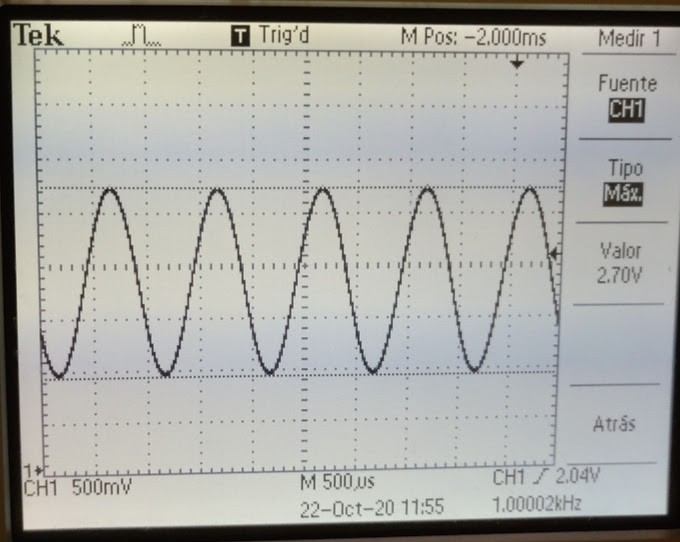
\includegraphics[scale=0.195]{max}
\end{center}

Valores medidos: $V_{medio}=1,79V$, $V_{min}=880mV$, $V_{max}=2,70V$. La amplitud de la onda es el valor: $|V_A|=V_{pp}/2=(V_{max}-V_{min})/2=(2,70-0,880)V/2=1,82V$ (en este caso, para $f=1kHz$.)

\bigskip

\textbf{A  continuación, represente en  el  osciloscopio únicamente  la  componente  alterna de  la tensión  en  el  nodo  A utilizando  el  modo  de  acoplamiento  AC. Varíe entonces la  frecuencia desde 50 Hz hasta 50 kHz ‘logarítmicamente’ tomando varios puntos por década (por ej. 50, 60, 70, 80, 90, 100, 200, ...800, 900, 1000, 2000, ... 8000, 9000, 10000, 20000, 30000, 40000, 50000) Realice las siguientes tareas para cada una de las frecuencias: }

\textbf{a) Mida la amplitud de la señal $V_A$.}

\textbf{b) Mida la amplitud de la señal de entrada V2 usando el Canal 2.}
 
\textbf{c) Mida el  desfase  temporal ($\delta t$)  entre  las  dos  ondas. Utilice  siempre  como referencia la misma onda.}

Datos obtenidos: (en la segunda columna se tiene el valor dado por el menú MEASURE, es decir, la $V_{pp}$, por lo que $V_A$ es la mitad.)

\begin{table}[h]
\centering
\begin{tabular}{|r|r|r|r|r|r|r|}
\hline
\multicolumn{1}{|l|}{frecuencia (Hz)} & \multicolumn{1}{l|}{$2|V_A|(V)$} & \multicolumn{1}{l|}{$|V_A|(V)$} & \multicolumn{1}{l|}{$|V_2|(V)$} & \multicolumn{1}{l|}{$|A_v|=\frac{|V_A|}{|V_2|}$} & \multicolumn{1}{l|}{$\delta t(s)$} & \multicolumn{1}{l|}{$\phi=2\pi f (\delta t)$ (rad)} \\
\hline
50    & 0,104 & 0,052 & 2    & 0,026         & 0,005      & 1,570796327   \\ \hline
60    & 0,128 & 0,064 & 2    & 0,032         & 0,004      & 1,507964474   \\ \hline
70    & 0,148 & 0,074 & 2    & 0,037         & 0,0036     & 1,583362697   \\ \hline
80    & 0,168 & 0,084 & 2    & 0,042         & 0,0031     & 1,558229956   \\ \hline
90    & 0,192 & 0,096 & 2,04 & 0,04705882353 & 0,0027     & 1,52681403    \\ \hline
100   & 0,208 & 0,104 & 2,04 & 0,05098039216 & 0,0023     & 1,445132621   \\ \hline
200   & 0,408 & 0,204 & 2    & 0,102         & 0,00116    & 1,457698991   \\ \hline
300   & 0,608 & 0,304 & 2,04 & 0,1490196078  & 0,00074    & 1,394867138   \\ \hline
400   & 0,796 & 0,398 & 2,04 & 0,1950980392  & 0,00052    & 1,306902544   \\ \hline
500   & 0,98  & 0,49  & 2    & 0,245         & 0,00043    & 1,350884841   \\ \hline
600   & 1,2   & 0,6   & 2,04 & 0,2941176471  & 0,00033    & 1,244070691   \\ \hline
700   & 1,34  & 0,67  & 2,04 & 0,3284313725  & 0,000292   & 1,284283077   \\ \hline
800   & 1,52  & 0,76  & 2,04 & 0,3725490196  & 0,00024    & 1,206371579   \\ \hline
900   & 1,66  & 0,83  & 2    & 0,415         & 0,000212   & 1,198831757   \\ \hline
1000  & 1,8   & 0,9   & 2    & 0,45          & 0,00018    & 1,130973355   \\ \hline
2000  & 2,78  & 1,39  & 2    & 0,695         & 0,000066   & 0,8293804605  \\ \hline
3000  & 3,22  & 1,61  & 2    & 0,805         & 0,000031   & 0,5843362336  \\ \hline
4000  & 3,46  & 1,73  & 1,96 & 0,8826530612  & 0,000018   & 0,4523893421  \\ \hline
5000  & 3,56  & 1,78  & 1,96 & 0,9081632653  & 0,0000126  & 0,3958406744  \\ \hline
6000  & 3,68  & 1,84  & 1,96 & 0,9387755102  & 0,0000095  & 0,3581415625  \\ \hline
7000  & 3,73  & 1,865 & 1,96 & 0,9515306122  & 0,0000063  & 0,277088472   \\ \hline
8000  & 3,84  & 1,92  & 1,96 & 0,9795918367  & 0,0000041  & 0,2060884781  \\ \hline
9000  & 3,92  & 1,96  & 1,96 & 1             & 0,000004   & 0,2261946711  \\ \hline
10000 & 3,92  & 1,96  & 1,96 & 1             & 0,0000039  & 0,245044227   \\ \hline
20000 & 4     & 2     & 2    & 1             & 0,0000012  & 0,1507964474  \\ \hline
30000 & 4     & 2     & 2    & 1             & 0,00000072 & 0,1357168026  \\ \hline
40000 & 4     & 2     & 2    & 1             & 0,00000037 & 0,09299114255 \\ \hline
50000 & 4     & 2     & 2    & 1             & 0,00000012 & 0,03769911184 \\ \hline

\end{tabular}
\end{table}
\begin{center}
{(Tabla 1)}
\end{center}
Nota: en los últimos valores tomados del valor $V_{pp}$ se observará luego en las gráficas que no se ajusta muy bien a la función (hay ciertos picos), esto se debe a que al tener los valores de tal tamaño, en el osciloscopio, un pequeño movimiento del cursor pasaba del valor 3,84V al 3,92V y directamente al 4,00V (aumentaba con una sensibilidad de 0,08V que no era suficiente para tomar con mucha precisión dichos valores).

\cleardoublepage

A continuación se muestran la pantalla del osciloscopio en la toma de datos para una de las frecuencias (300Hz).

\begin{center}
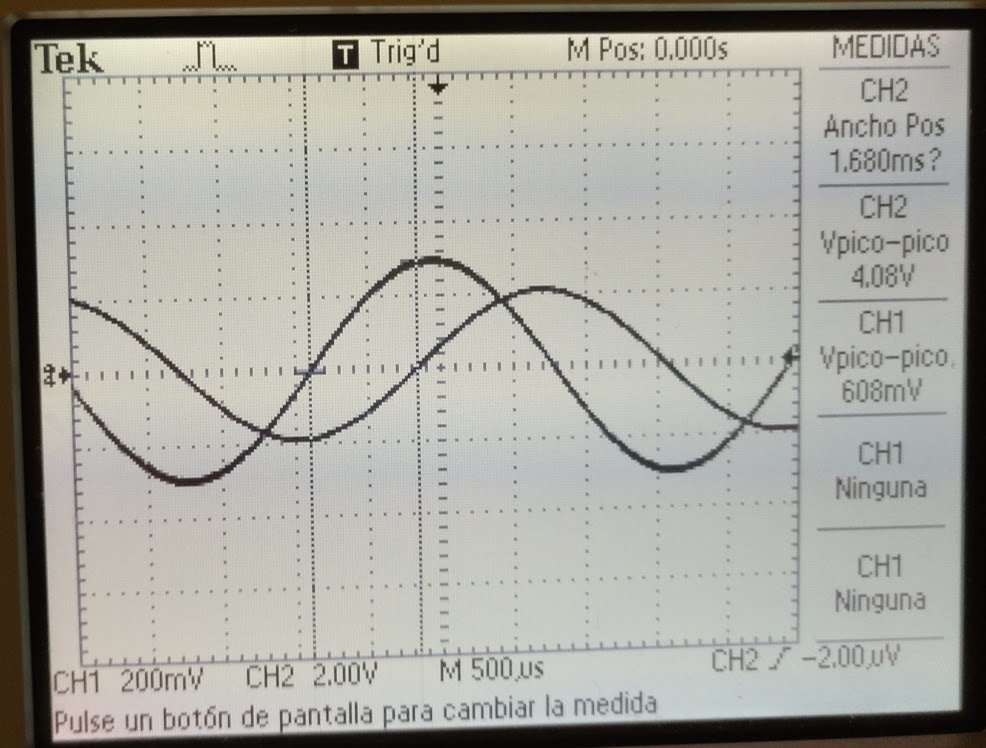
\includegraphics[scale=0.2925]{f300v}\\
\end{center}
Aquí se tiene la medida del valor pico-pico, utilizando el menú MEASURE del osciloscopio, nos fijamos en el CH1. Podemos observar también, que el Vpico-pico del CH2, que mide  $V_2$, no es exactamente 4,00V. Durante las mediciones ha estado variando entre 4,08V y 3,92V; a causa de lo cual, se producirán más errores en las medidas.\\
\begin{center}
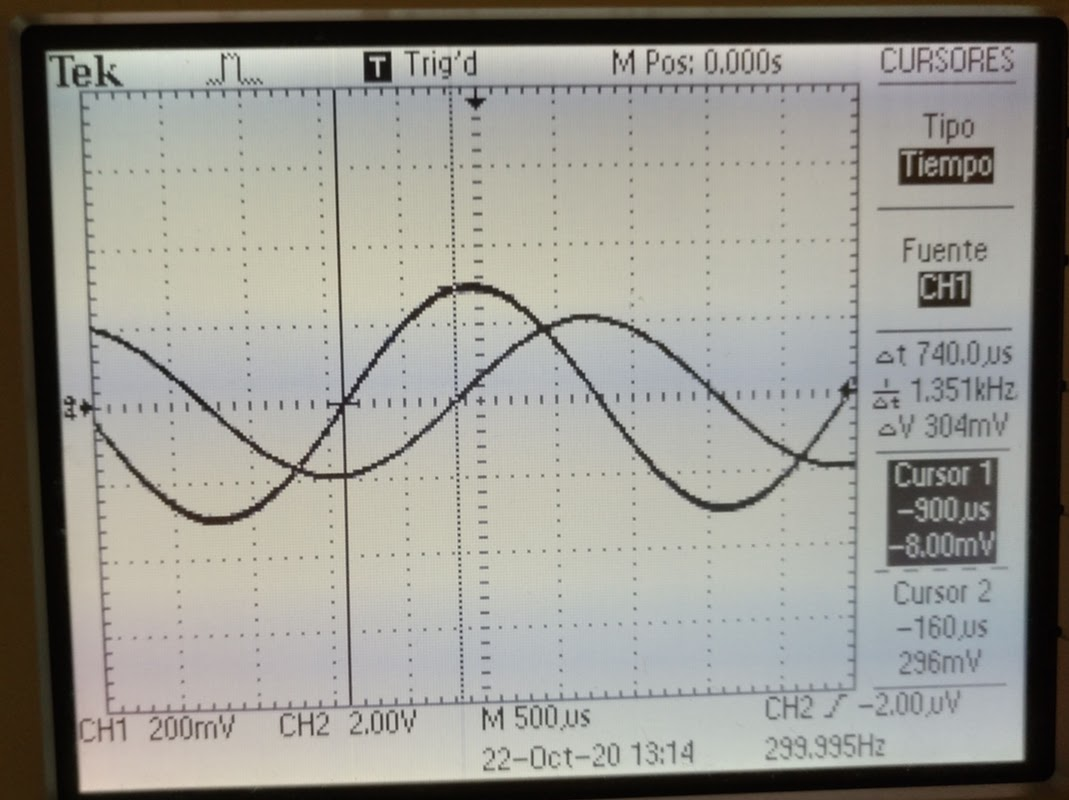
\includegraphics[scale=0.27]{f300t}\\
\end{center}
En este caso, se ha medido el desfase temporal con los cursores, utilizando el corte de las dos gráficas con el eje x. Esta medición con los cursores ha sido especialmente difícil de llevar a cabo con precisión, ya que, aunque se ampliara la gráfica, los trazos eran tan gruesos que no se veía bien dónde se producía exactamente la intersección con los ejes. Y esta dificultad se ha ido haciendo mayor a medida que las frecuencias aumentaban.


\cleardoublepage

\textbf{a) Represente $A_v$ en escala lineal ($|V_A|/|V_2|$) y en decibelios ($20 \log (|V_A|/|V_2|)$) en función de la frecuencia usando una escala logarítmica para el eje X. Compruebe que el circuito se comporta como un filtro paso alto.}

Nota: estas gráficas se han realizado con Gnuplot.

\begin{center}
\includegraphics[scale=0.65]{g}\\
Gráfica representado $|Av|$ (adimensional).\\
\bigskip
\bigskip
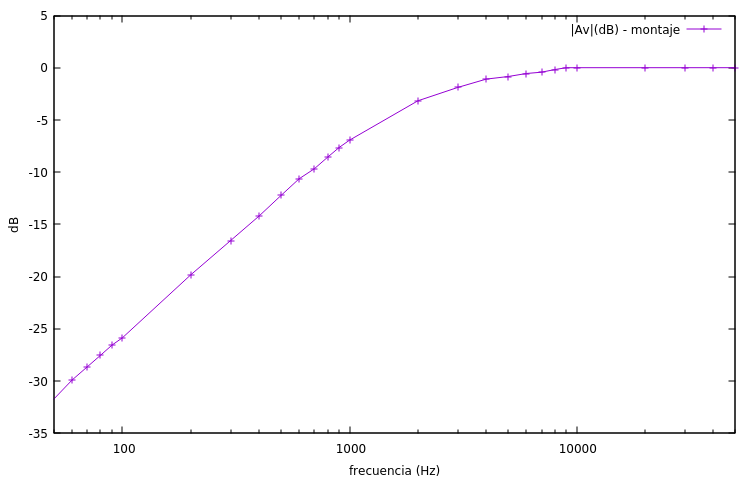
\includegraphics[scale=0.65]{g_db}\\
Gráfica representando $20 \log (|Av|)$ - (en dB).
\end{center}

Como podemos ver en la gráfica, cuando $f\rightarrow 0$, $|A_v|\rightarrow 0$. Y cuando $f\rightarrow \infty$, $|A_v|\rightarrow 1$. Por lo que se comporta como un fitro de paso alto.

\cleardoublepage
\textbf{b) Convierta el  desajuste  temporal  en  diferencia  de  fase  en  grados  o  radianes utilizando la siguiente expresión:
$$\delta t/T=\phi /360^o=\phi /(2\pi rad)$$
donde $T$ es el periodo de la señal. Represente la diferencia de fase en función de la frecuencia usando una escala logarítmica para el eje X.}\\

\bigskip

De la expresión obtenemos que $\phi = 2\pi.f.\delta t $ - estos datos se han incluido en la tabla de los datos obtenidos en la práctica (Tabla 1).

\begin{center}
\includegraphics[scale=0.7]{fase_fea}
\end{center}

\textbf{c) Compare los resultados con los obtenidos del análisis teórico del circuito y de los trabajos de simulación.}

En el trabajo previo, se observó que los valores de la simulación eran prácticamente los mismos que los teóricos. En el trabajo previo, se calculó que 

\[|A_v|(f)=\frac{1}{\sqrt{1+\left(\frac{1}{2\pi f C R_{eq}}\right)^2}}\]

donde $C=100nF$ y $R_{eq}=824,56\Omega.$%imagen gan_vs_teo
\cleardoublepage
A continuación se muestra la gráfica en la que se compara la función $|A_v|(f)$ calculada teóricamente, con la gráfica de los datos recogidos en el montaje. (En este caso no se muestran los puntos con cruces para facilitar la visualización.)

\begin{center}
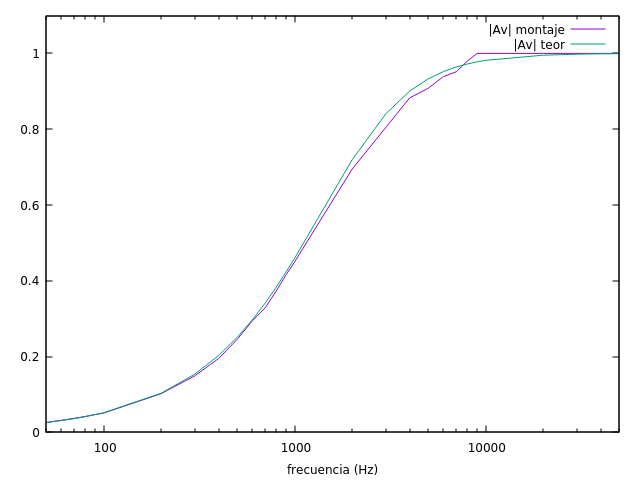
\includegraphics[scale=0.6]{g_v_t}
\end{center}

En esta gráfica se aprecia la desviación que se tiene especialmente en los valores a partir de $2000$Hz con respecto a la función teórica, los valores tomados en el montaje son en todo momento ligeramente inferiores. Sin embargo, para los valores más altos, la función teórica tiende a 1, pero llega un punto en el que los valores la superan. Esto se debe, como se comentó al pie de la Tabla 1, a que para estas frecuencias tan altas, el Vpico-pico de la onda $V_A$ se podían tomar únicamente con una precisión de $0,08V$, por lo cual, se perdía bastante exactitud en estos valores, especialmente para que se pueda notar la sutileza de una función suave aproximándose a una asíntota, como sí vemos que hace la función teórica.

Gráfica de las mismas funciones (ganancias teóricas y del montaje en el nodo A) en dB:
\begin{center}
\includegraphics[scale=0.6]{g_v_tdb}
\end{center}

El valor teórico de la fase correspondía a:
$$\phi (f)= - \arctan\left(\frac{-1}{2\pi C R_{eq} f}\right)$$

En la siguiente gráfica se muestra dicha función $\phi (f)$ junto con los valores de la fase que se han calculado a partir de las medidas en el montaje del desfase temporal entre $V_A$ y $V_2$.

\begin{center}
\includegraphics[scale=0.55]{fasevt}
\end{center}

A pesar de que los valores se ajustan a lo esperado, esta vez sí que podemos observar grandes variaciones; principalmente ocasionadas, en mi opinión, por las dificultades que suponía el tener que medir los dafases temporales con los cursores del osciloscopio, unido al ruido que había en las ondas, que hacía que estas tuvieran un gran grosor, como se ha comentado ya en  el apartado de la toma de datos (página 3). 

\bigskip

\textbf{d) Determine la frecuencia de corte y compare con el valor teórico.}

La frecuencia de corte no se pidió en el trabajo previo. Sin embargo, el cálculo teórico en este caso es rápido:

$$|A_v|(f)=\frac{1}{\sqrt{1+\left(\frac{1}{2\pi f C R_{eq}}\right)^2}}$$
\bigskip
$$|A_v|(f)=\frac{1}{\sqrt 2} \iff f=f_c=\frac{1}{2\pi C R_{eq}} = \frac{1}{2\pi . 100 nF .824,56\Omega} \approx 1930,18 Hz$$
\bigskip

Como ya hemos visto en el apartado (c), los valores obtenidos del módulo de la ganancia son un poco menores que los calculados teóricamente. En los valores del montaje, se observa que $|A_v|$ tiene un valor de $\frac{1}{\sqrt 2}\approx 0,7071$, cuando la frecuencia es aproximadamente 2000Hz (ya que con 2000 Hz, la ganancia que hemos recogido es de valor 0,695), por lo que una vez más, la ganancia recogida es ligeramente inferior a la esperada. 

En la siguiente imagen se puede ver la intersección entre $\frac{1}{\sqrt 2}$ y la gráfica de los valores del montaje:

\begin{center}
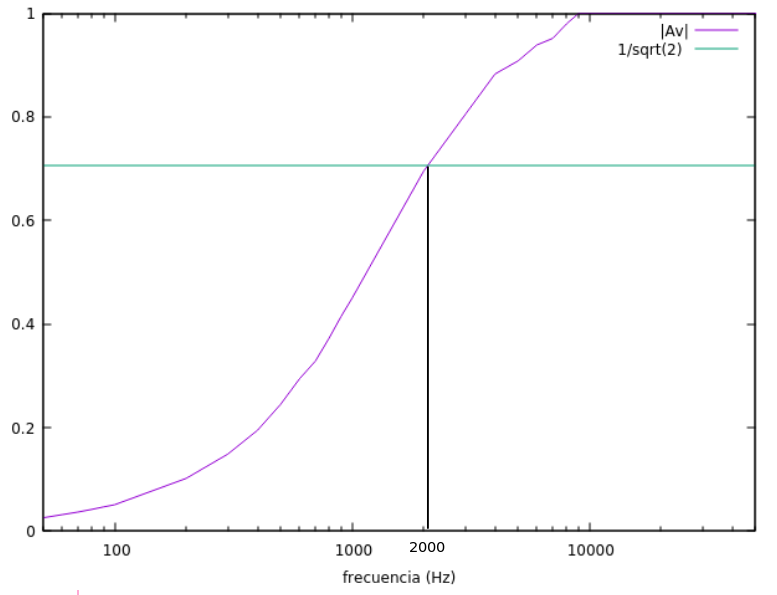
\includegraphics[scale=0.3]{f_c}
\end{center}

Podemos también buscar la frecuencia de corte también entre los valores de la fase (aunque hemos visto que son más imprecisos), ya que sabemos que 
$$f_c=  \frac{1}{2\pi C R_{eq}} \Longrightarrow \phi (f_c) = - \arctan\left(\frac{-1}{2\pi C R_{eq} f_c}\right) = -\arctan \left(\frac{-f_c}{f_c}\right) = \frac{\pi}{4} \approx 0,7854$$

De las fases que hemos calculado empíricamente, la que más se aproxima a este valor es la correspondiente a la frecuencia de 2000Hz, donde se tiene que la fase es 0,8293804605 rad. (La de 1000Hz es 1,13 rad, y la de 3000Hz es de 0,58 rad).

\end{document}